\section{Diagrama de Actividades}
\begin{center}
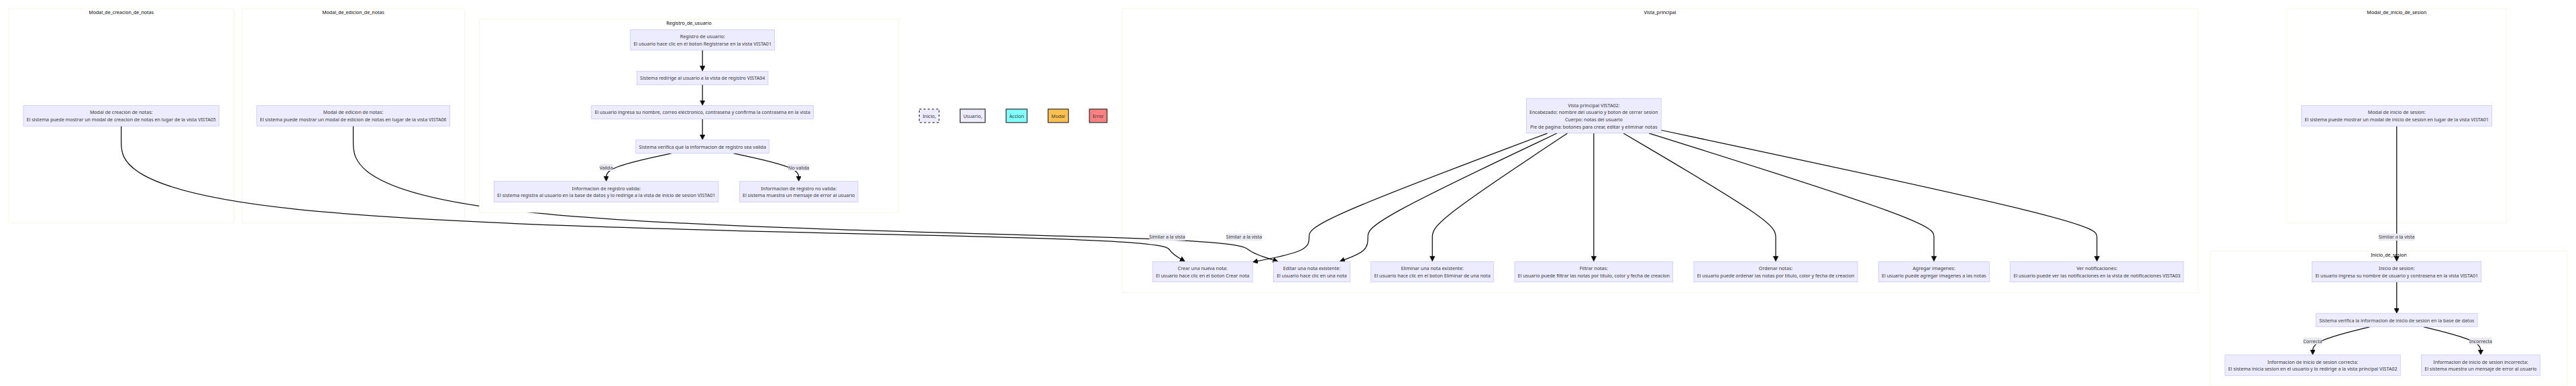
\includegraphics[width=0.8\textwidth]{IMA/Diagrama de Actividades3.png}
\end{center}

\section{Casos de Uso}
\subsection{Crear Nota}
\subsubsection{Actor Principal}
Usuario

\subsubsection{Descripción}
El usuario crea una nueva nota en el tablero.

\begin{enumerate}
  \item El usuario selecciona la opción "Crear Nota" en la interfaz de la aplicación.
  \item La aplicación muestra un formulario donde el usuario puede ingresar el título y contenido de la nueva nota.
  \item El usuario ingresa el título y contenido de la nota y confirma la creación.
  \item La aplicación guarda la nueva nota en el tablero y la muestra al usuario.
\end{enumerate}

\subsection{Editar Nota}
\subsubsection{Actor Principal}
Usuario

\subsubsection{Descripción}
El usuario edita una nota existente en el tablero.

\begin{enumerate}
  \item El usuario selecciona la nota que desea editar en el tablero.
  \item La aplicación muestra el contenido de la nota y ofrece la opción de edición.
  \item El usuario realiza los cambios deseados en el título o contenido de la nota.
  \item El usuario confirma los cambios y la aplicación guarda la nota actualizada en el tablero.
\end{enumerate}

\subsection{Eliminar Nota}
\subsubsection{Actor Principal}
Usuario

\subsubsection{Descripción}
El usuario elimina una nota del tablero.

\begin{enumerate}
  \item El usuario selecciona la nota que desea eliminar en el tablero.
  \item La aplicación muestra la opción de eliminar la nota.
  \item El usuario confirma la eliminación de la nota.
  \item La aplicación elimina la nota del tablero y actualiza la vista.
\end{enumerate}

\subsection{Organizar Notas}
\subsubsection{Actor Principal}
Usuario

\subsubsection{Descripción}
El usuario organiza las notas en el tablero según su preferencia.

\begin{enumerate}
  \item El usuario selecciona y arrastra una nota a una nueva posición en el tablero.
  \item La aplicación actualiza la posición de la nota en el tablero según el movimiento del usuario.
  \item El usuario suelta la nota en la nueva posición y la aplicación confirma la actualización.
\end{enumerate}

\begin{center}
    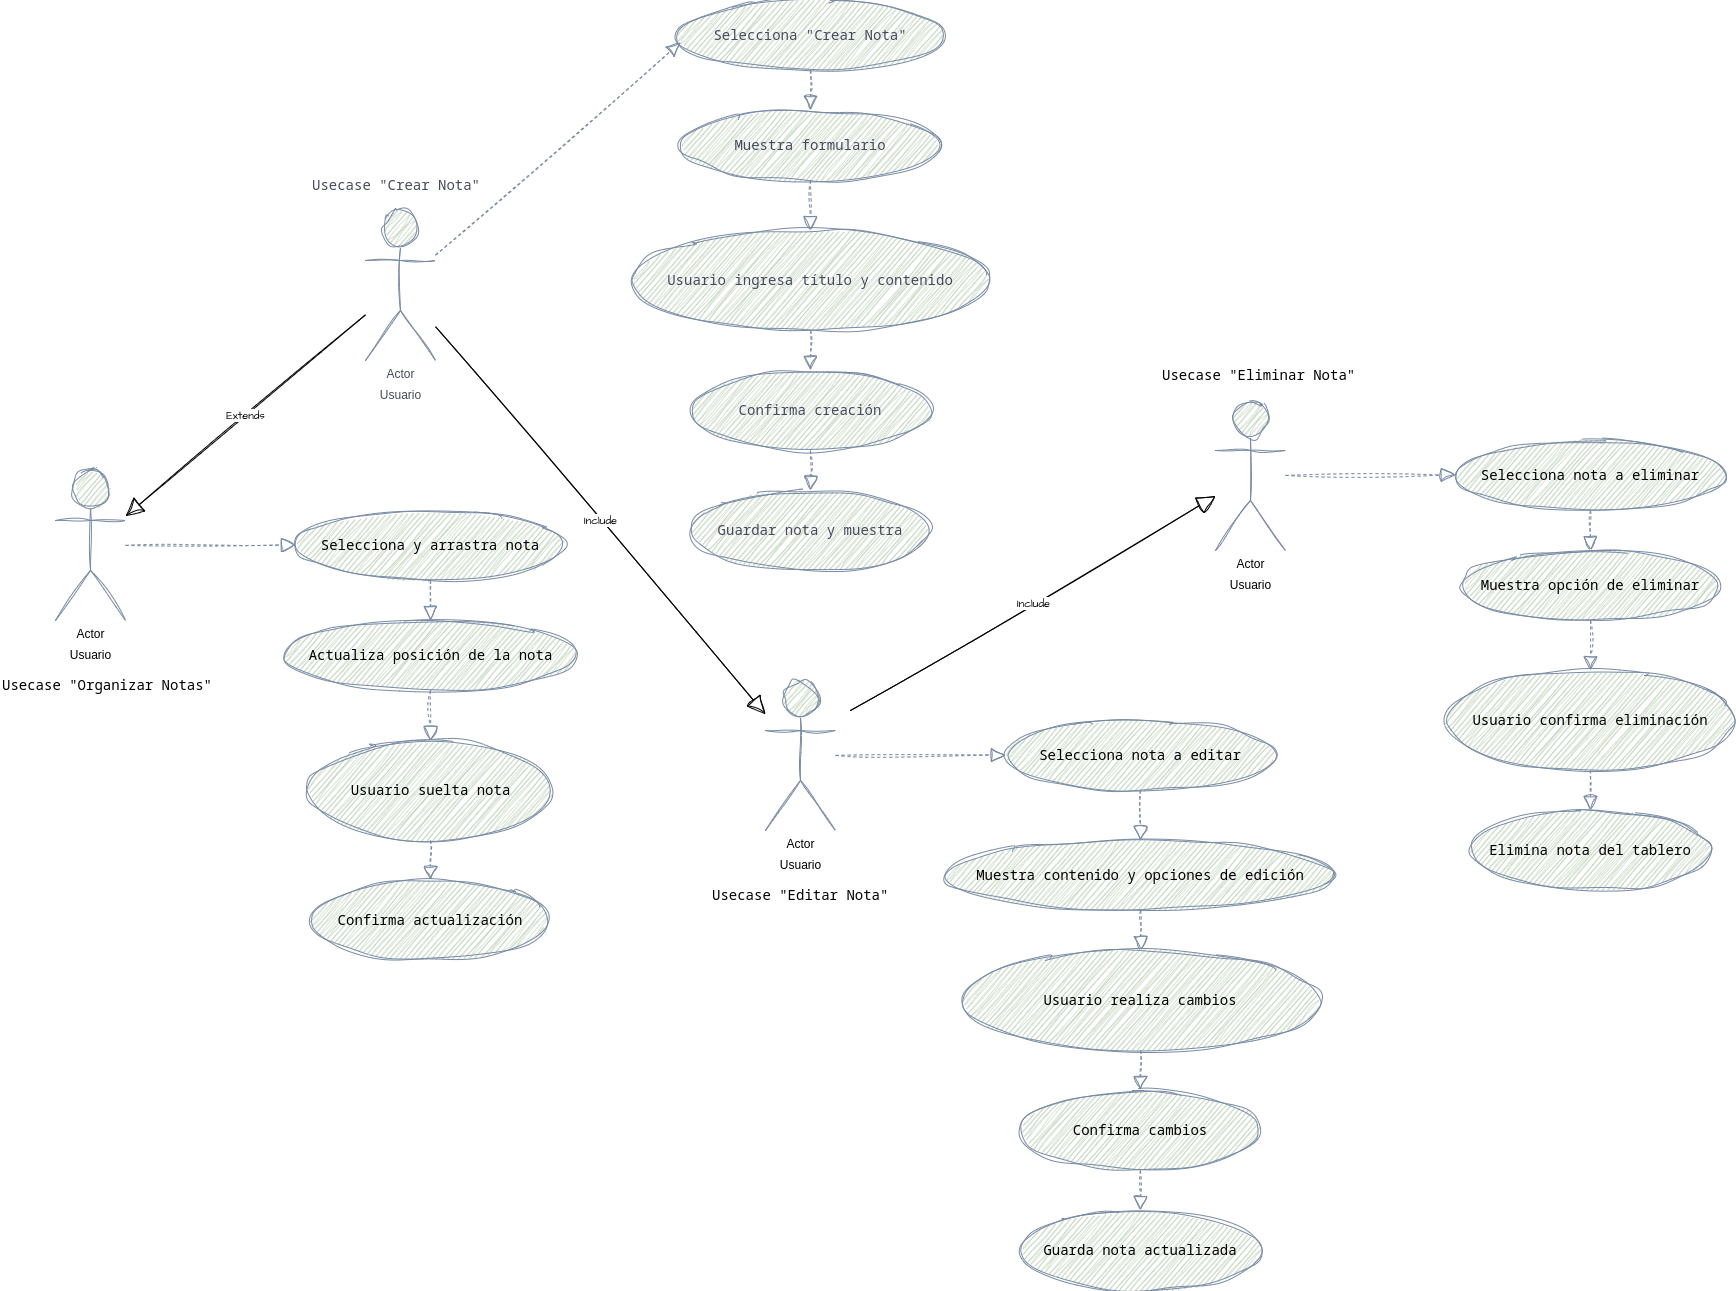
\includegraphics[scale = .20]{IMA/CasosUso.drawio.png}
\end{center}
